\documentclass[11pt, a4paper]{article}

\usepackage{tikz}
\usetikzlibrary{shapes,arrows}
\usepackage{placeins}
\usepackage{amsmath}
\usepackage{mathrsfs}
\usepackage{bm}
\usepackage{amssymb}

\begin{document}

\title{SUPPORT VECTOR MACHINES}
\date{}
\maketitle

Support Vector Machines (SVMs) are one of the most powerful supervised learning algorithms which work on the idea of finding the `safest' separator hyperplane (one with the largest `margin') to divide the labelled hyperspace.

\section{Optimal Linear Separator}

Given training data of the form $(x_1, y_1),\ (x_2, y_2),\ ...\ , (x_n, y_n)$ where $y_i \in \{+1, -1\}\ \forall\ x_i \in \mathbf{X}$, what is the optimal linear separator that can separate the positives from the negatives?

\begin{figure}[htbp]
	\centering
	\begin{tikzpicture}
		\tikzstyle {point line} = [line width=0.15em]
		\tikzstyle {margin} = [dashed]
						    
		\draw[-latex] (0,0) -- (6,0) node[right]{};
		\draw[-latex] (0,0) -- (0,5) node[left]{};	
				
		\draw[point line] (1.7, 1) -- (2.3, 1);	
		\draw[point line] (.7, 2) -- (1.3, 2);
				
		\draw[point line] (2.7, 3) -- (3.3, 3);
		\draw[point line] (3, 2.7) -- (3, 3.3);					
		
		\draw[point line] (2.7, 4) -- (3.3, 4);
		\draw[point line] (3, 3.7) -- (3, 4.3);	
			    
		\draw[point line] (3.7, 3) -- (4.3, 3);
		\draw[point line] (4, 2.7) -- (4, 3.3);
			    
		\draw[margin] (4, 0.5) -- (.5, 4);
		\draw (4, 0.5) node [below right] {$H_1$};    					
		
		\draw[margin] (2.5, 4.5) -- (2.5, 0.5);
		\draw (2.5, 0.5) node [below] {$H_2$};    							
	\end{tikzpicture}
\end{figure}

It is clear that $H_1$ is a better linear separator as opposed to $H_2$. It is expected that $H_1$ will make fewer errors for predicting unseen points as comapred to $H_2$.

\section{Derivation}

Let $\vec{\mathbf{w}}$ be a vector perpendicular to a linear separator. The following figure visualizes the constraint that the separator is subjected to.

\FloatBarrier\clearpage
\begin{figure}[htbp]
	\centering
	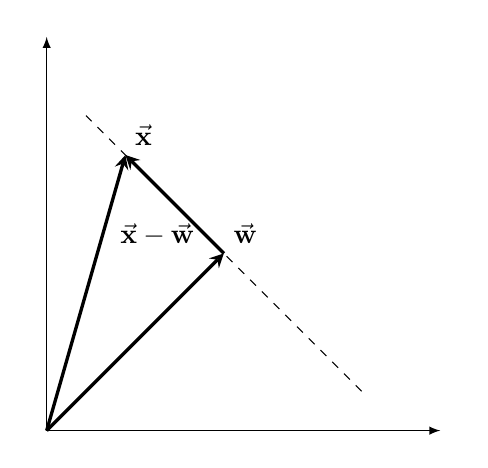
\begin{tikzpicture}
		\tikzstyle {margin} = [dashed]
		\tikzstyle {vector} = [very thick,->, >=stealth]
						    
		\draw[-latex] (0,0) -- (5,0) node[right]{};
		\draw[-latex] (0,0) -- (0,5) node[left]{};	
				
		\draw[margin] (4, 0.5) -- (.5, 4);
				
		\draw[vector] (0, 0) -- (2.25, 2.25);
		\draw (2.25, 2.25) node [above right] {$\vec{\mathbf{w}}$};    	
				
		\draw[vector] (0, 0) -- (1, 3.5);
		\draw (1, 3.5) node [above right] {$\vec{\mathbf{x}}$};
				
		\draw[vector] (2.25, 2.25) -- (1, 3.5);
		\draw (2, 2.75) node [below left] {$\vec{\mathbf{x}} - \vec{\mathbf{w}}$};
				   							
	\end{tikzpicture}
\end{figure}

\begin{align*}
	(\vec{\mathbf{x}} - \vec{\mathbf{w}}).\vec{\mathbf{w}} = 0   \\
	\vec{\mathbf{x}}.\vec{\mathbf{w}} - |\vec{\mathbf{w}}|^2 = 0 \\
	\vec{\mathbf{x}}.\vec{\mathbf{w}} - b = 0                    \\
\end{align*}

Assume two hyperplanes parallel to the separator hyperplane, one on each side of the separator, such that they cut through the closest training point(s) on the corresponding side. The equations for these `support' hyperplanes are,

\begin{align*}
	\vec{\mathbf{x_{+}}}.\vec{\mathbf{w}} = b + \delta \\
	\vec{\mathbf{x_{-}}}.\vec{\mathbf{w}} = b - \delta \\
\end{align*}

Note that the subscipts $+$ and $-$ denote the positive and negative side respectively. The equations are still satisfied if we scale $\vec{\mathbf{w}}$ and ($b$ and $\delta$) by the same amount. Hence, $\delta = 1$ is set to avoid this difficutly. 

\begin{align*}
	\vec{\mathbf{x_{+}}}.\vec{\mathbf{w}} = b + 1 \\
	\vec{\mathbf{x_{-}}}.\vec{\mathbf{w}} = b - 1 \\
\end{align*}

The length of margin between the $+$ support hyperplane and the $-$ support hyperplane is calculated as follows, 

\begin{align*}
	margin & = (\vec{\mathbf{x_{+}}} - \vec{\mathbf{x_{-}}}) . \frac{\vec{\mathbf{w}}}{|\vec{\mathbf{w}}|} \\
	       & = \frac{2}{|\vec{\mathbf{w}}|}                                                                \\    
\end{align*}

All positive and negative points can be assumed to follow, 

\begin{align*}
	\vec{\mathbf{x_{+}}}.\vec{\mathbf{w}} \geq b + 1 \\
	\vec{\mathbf{x_{-}}}.\vec{\mathbf{w}} \leq b - 1 \\    
\end{align*}

These equations can be combined together to form,

\begin{align*}
	y \times (\vec{\mathbf{x}}.\vec{\mathbf{w}} - b) - 1 \geq 0 \\
\end{align*}

or, 

\begin{align*}
	y_i \times (\vec{\mathbf{x_i}}.\vec{\mathbf{w}} - b) - 1 \geq 0\ \forall\ i \\
\end{align*}

The problem can be formulated as follows,

\begin{align*}
	\text{maximize}\ \frac{2}{\vec{\mathbf{|w|}}}\ \text{subject to}\           
	y_i \times (\vec{\mathbf{x_i}}.\vec{\mathbf{w}} - b) - 1 \geq 0\ \forall\ i \\
\end{align*}

or, 

\begin{align*}
	\text{minimize}\ \frac{1}{2} \times {\vec{\mathbf{|w|}}^2}\ \text{subject to}\ 
	y_i \times (\vec{\mathbf{x_i}}.\vec{\mathbf{w}} - b) - 1 \geq 0\ \forall\ i    \\
\end{align*}

This form is called the primal form and it is a quadratic optimization problem but not readily kernelized. The primal form is converted the dual form by using a Langrangian.

\begin{align*}
	\mathscr{L}(\vec{\mathbf{w}},\ b,\ \bm{\alpha}) = \frac{1}{2} \times \vec{\mathbf{|w|}}^2 - \sum\limits_{i = 1}^N \alpha_i \times [ y_i \times (\vec{\mathbf{x_i}}.\vec{\mathbf{w}} - b) - 1 ] 
\end{align*}

Taking derivative w.r.t $\vec{\mathbf{w}}$ and $b$, equating to zero and solving, these two equations arise.

\begin{align}
	\vec{\mathbf{w}}^*                        & = \sum\limits_{i = 1}^N \alpha_i \times y_i \times \vec{\mathbf{x_i}} \\
	\sum\limits_{i = 1}^N \alpha_i \times y_i & = 0                                                                   
\end{align}

Now, for a point $i$ on a support hyperplane, 

\begin{align*}
	y_i \times (\vec{\mathbf{x_i}}.\vec{\mathbf{w}}^* - b^*) = 1              \\
	y_i \times y_i \times (\vec{\mathbf{x_i}}.\vec{\mathbf{w}}^* - b^*) = y_i \\    
	\vec{\mathbf{x_i}}.\vec{\mathbf{w}}^* - b^* = y_i                         \\
	b^* = y_i - \vec{\mathbf{x_i}}.\vec{\mathbf{w}}^*                         
\end{align*}

Inserting (1) and (2) back into langragian, the dual form takes the form of,

\begin{align*}
	\text{maximize}\ \mathscr{L}(\vec{\mathbf{w}},\ b,\ \bm{\alpha}) & = \sum\limits_{i = 1}^N \alpha_i                                                                                                            \\ 
	                                                                 & \ \ \ - \frac{1}{2} \times \sum\limits_{i, j} \alpha_i \times \alpha_j \times y_i \times y_j \times \vec{\mathbf{x_i}} . \vec{\mathbf{x_j}} \\
	\text{subject to}\ \sum\limits_{i = 1}^N \alpha_i \times y_i     & = 0\ \ \ \text{and}                                                                                                                         \\
	\alpha_i                                                         & >= 0\ \forall\ i                                                                                                                            
\end{align*}

The dual formation is also a quadratic optimization problem but is readily kernelized through the substitution $\vec{\mathbf{x_i}} . \vec{\mathbf{x_j}} \rightarrow k(\mathbf{x_i}, \mathbf{x_j})$.

The primal problem is convex and the dual formation is concave and due to duality theroy the duality gap is zero meaning the solutions for both (minima for primal and maxima for dual) the problems are the same.

An interesting equation which holds at the solution is,

\begin{align*}
	\alpha_i \times [y_i \times (\vec{\mathbf{x_i}}.\vec{\mathbf{w}} - b) - 1] = 0\ \forall\ i 
\end{align*}

At the points not on the support hyperplanes, $y_i \times (\vec{\mathbf{x_i}}.\vec{\mathbf{w}} - b) - 1 > 0$ or $y_i \times (\vec{\mathbf{x_i}}.\vec{\mathbf{w}} - b) - 1 < 0$ and hence $\alpha_i$ must be zero for each such point. On the other hand, for the points on the support hyperplanes, $y_i \times (\vec{\mathbf{x_i}}.\vec{\mathbf{w}} - b) - 1 = 0$ so $\alpha_i \geq 0$ for each such point. 

The training vectors on the support hyperplanes for which $\alpha_i > 0$ are called support vectors.

\section{Non Linearly Separable Case}

The equations for the non separable case are, 

\begin{align*}
	\vec{\mathbf{x_{i}}}.\vec{\mathbf{w}} & \geq b + 1 - \epsilon_i\ \forall\ y_i = +1 \\
	\vec{\mathbf{x_{i}}}.\vec{\mathbf{w}} & \leq b - 1 + \epsilon_i\ \forall\ y_i = -1 \\ 
	\epsilon_i                            & \geq 0\ \forall\ i                         
\end{align*}

The variables $\epsilon_i$s allow for violation of the constraint. Hence, we must penalize for that. One penalty function is $C \times \sum\limits_i \epsilon_i$ where C is the tradeoff between margin and penalty. To be on the wrong side of the hyperplane $\epsilon_i$ will be greater than one, so $\sum\limits_i \epsilon_i$ is an upper bound on number of violations.

The primal problem thus becomes,

\begin{align*}
	\text{minimize}\ \frac{1}{2} \times {\vec{\mathbf{|w|}}^2} + C \times \sum\limits_i \epsilon_i &                    \\ \text{subject to}\ y_i \times (\vec{\mathbf{x_i}}.\vec{\mathbf{w}} - b) - 1 + \epsilon_i &\geq 0\ \forall\ i\ and \\
	\epsilon_i                                                                                     & \geq 0\ \forall\ i 
\end{align*}

The dual formulation is also surprisingly similar,

\begin{align*}
	\text{maximize}\ \mathscr{L}(\vec{\mathbf{w}},\ b,\ \bm{\alpha}) & = \sum\limits_{i = 1}^N \alpha_i                                                                                                            \\ 
	                                                                 & \ \ \ - \frac{1}{2} \times \sum\limits_{i, j} \alpha_i \times \alpha_j \times y_i \times y_j \times \vec{\mathbf{x_i}} . \vec{\mathbf{x_j}} \\
	\text{subject to}\ \sum\limits_{i = 1}^N \alpha_i \times y_i     & = 0\ \ \ \text{and}                                                                                                                         \\
	0 <= \alpha_i                                                    & <= C\ \forall\ i                                                                                                                            
\end{align*}

The multipliers $\alpha_i$s are now constrained by C. Note that the dual formation is still readily kernelized.

\section*{The Kernel Trick}

Kernel functions are functions which let you calculate dot product in higher dimensions given vectors in lower dimensions. Sincel SVMs use only dot products, kernel function effectively solve the problem in higher dimensions without expliclity transforming each point into the higher dimension. This leads SVMs to be very time efficient algorithms even when solving the problem in higher dimensions than the input space.

Say there is a $\mathbb{R}^2 \rightarrow \mathbb{R}^3$ transformation function $\phi$ such that $\phi(i, j) = (i^2, \sqrt{2} \times i \times j, j^2)$, the kernel function $K(\vec{\mathbf{x}}, \vec{\mathbf{z}}) = (\vec{\mathbf{x}}.\vec{\mathbf{z}})^2$ works because,

\begin{align*}
	\phi(\vec{\mathbf{x}}).\phi(\vec{\mathbf{z}}) & = (x_i^2, \sqrt{2} \times x_i \times x_j, x_j^2).(z_i^2, \sqrt{2} \times z_i \times z_j, z_j^2) \\
	                                              & = x_i^2 \times z_i^2 + 2 \times x_i \times x_j \times z_i \times z_j + x_j^2 \times z_j^2       \\
	                                              & = (x_i \times z_i + x_j \times z_j)^2                                                           \\
	                                              & = (\vec{\mathbf{x}}.\vec{\mathbf{z}})^2                                                         \\
	                                              & = K(\vec{\mathbf{x}}, \vec{\mathbf{z}})                                                         \\
\end{align*}

\section{Comments}

\begin{itemize}
	\item SVMs are helpful in tasks like text classification, image classification, digit recognition etc.
	\item SVMs can work with limited amount of training data and high dimensional data effectively.
	\item The maximal margin approach reduces overfitting allowing SVMs to generalize better.
	\item SVMs are typically quite robust against noise.
\end{itemize} 

\end{document}